\documentclass[conference, 10pt]{IEEEtran}

% ─── Packages ──────────────────────────────────────────────────────
\usepackage{amsmath,amssymb,amsfonts}
\usepackage{graphicx}
\usepackage{textcomp}
\usepackage{xcolor}
\usepackage{booktabs}
\usepackage{algorithm}
\usepackage{algpseudocode}
\usepackage{subcaption}
\usepackage{hyperref}
\usepackage{cite}
\usepackage{multirow}
\usepackage{array}
\usepackage{enumitem}
\usepackage{tikz}
\usepackage{colortbl}
\usepackage{makecell}

% ─── Colors ────────────────────────────────────────────────────────
\definecolor{dqnblue}{HTML}{1565C0}
\definecolor{lfagreen}{HTML}{2E7D32}
\definecolor{ppoorange}{HTML}{E65100}
\definecolor{grpopurple}{HTML}{6A1B9A}
\definecolor{highlight}{HTML}{FFF3E0}
\definecolor{lightgray}{HTML}{F5F5F5}

% ─── Compact spacing ──────────────────────────────────────────────
\setlength{\textfloatsep}{6pt plus 2pt minus 2pt}
\setlength{\floatsep}{6pt plus 2pt minus 2pt}
\setlength{\intextsep}{6pt plus 2pt minus 2pt}
\setlength{\abovecaptionskip}{4pt}
\setlength{\belowcaptionskip}{2pt}

\begin{document}

% ═══════════════════════════════════════════════════════════════════
% PAGE 1: Title, MDP, Architecture
% ═══════════════════════════════════════════════════════════════════

\title{\LARGE Solving 2048: Classical RL vs.\ LLM-Guided RLVR\\[4pt]
\large A Comparative Study of Seven Reinforcement Learning Agents}

\author{
\IEEEauthorblockN{Shriman Raghav \quad Gautham Ramkumar}
\IEEEauthorblockA{
\textit{MS Robotics, Khoury College of Computer Sciences}\\
\textit{Northeastern University}, Boston, MA\\
\texttt{srinivasan.shrim@northeastern.edu}}
}

\maketitle
\thispagestyle{plain}

% ──────────────────────────────────────────────────────────────────
\section{Introduction}
% ──────────────────────────────────────────────────────────────────

The puzzle 2048 is a compelling RL benchmark combining stochastic dynamics, a combinatorial state space ($\sim\!10^{19}$ configurations), and sparse, delayed rewards.  We conduct the first controlled comparison of six classical RL agents and an LLM fine-tuned with Group Relative Policy Optimization (GRPO), a form of Reinforcement Learning with Verifiable Rewards (RLVR).

\textbf{Research questions.}
\textbf{(Q1)}~How do five modern RL algorithms compare when architectural confounds are removed?
\textbf{(Q2)}~Can a 0.5B-parameter LLM learn 2048 strategy through GRPO alone?
\textbf{(Q3)}~How does sample efficiency scale from 1M to 5M training steps?

% ──────────────────────────────────────────────────────────────────
\section{MDP Formulation}
\label{sec:mdp}
% ──────────────────────────────────────────────────────────────────

We formalize 2048 as an MDP $\langle \mathcal{S}, \mathcal{A}, \mathcal{T}, \mathcal{R}, \gamma \rangle$:

\subsection{State Space $\mathcal{S}$}
The raw state is a $4{\times}4$ board $B\!\in\!\mathbb{Z}_{\geq 0}^{4\times 4}$, where each cell holds a tile value $\in\{0,2,4,...,2^{15}\}$.  For CNN agents, we encode it as a 16-channel binary tensor $\mathbf{x}\!\in\!\{0,1\}^{16\times 4\times 4}$:
\begin{equation}
    x_{k,i,j}=\mathbb{1}\!\left[B_{i,j}=2^{k}\right],\quad k=0,1,\dots,15
    \label{eq:obs}
\end{equation}
Channel~0 marks empty cells; channel~$k$ marks tiles of value~$2^k$, avoiding magnitude bias in convolutions.  For the LLM agent, $B$ is serialized as a labeled ASCII grid.

\subsection{Action Space $\mathcal{A}$}
$\mathcal{A}=\{0,1,2,3\}$ mapping to $\{\text{UP},\text{RIGHT},\text{DOWN},\text{LEFT}\}$.

\subsection{Transition $\mathcal{T}(s'\mid s,a)$}
Each transition has a deterministic component (slide \& merge tiles) and a stochastic component (spawn a 2-tile with $p{=}0.9$ or 4-tile with $p{=}0.1$ at a random empty cell).  If action $a$ produces no board change, it is \emph{invalid}---no tile spawns.  The game terminates when no action changes the board.

\subsection{Reward $\mathcal{R}(s,a,s')$}
\begin{equation}
r = \begin{cases}
\Delta\text{score} + \text{milestones} & \text{(shaped mode)} \\
-1 & \text{(invalid move)}
\end{cases}
\end{equation}
where milestones are one-time bonuses: $+50$ at tile~256, $+100$ at 512, $+200$ at 1024, $+500$ at 2048.  Discount factor $\gamma{=}0.99$.

\vspace{2pt}
\noindent\fbox{\parbox{0.96\columnwidth}{\small
\textbf{Why 2048 is hard:}
(1)~Sparse, delayed rewards---hundreds of merges precede a single high-value event;
(2)~Stochastic tile spawns prevent deterministic planning;
(3)~$\sim\!10^{19}$ states make tabular methods infeasible;
(4)~Episodes last 100--1000+ steps.
}}

% ──────────────────────────────────────────────────────────────────
\section{Architecture \& Agents}
\label{sec:agents}
% ──────────────────────────────────────────────────────────────────

\subsection{Shared CNN Backbone}
Every deep classical agent shares an identical 3-layer CNN feature extractor $\phi_\theta$ to isolate the effect of the learning \emph{algorithm}:
\begin{equation}
\phi_\theta:\; \mathbb{R}^{16\times 4\times 4}
\!\xrightarrow{\text{Conv}_{128}^{2\times 2}}
\!\xrightarrow{\text{Conv}_{128}^{2\times 2}}
\!\xrightarrow{\text{Conv}_{128}^{2\times 2}}
\!\xrightarrow{\text{FC}_{256}}
\mathbb{R}^{256}
\end{equation}
Each algorithm appends task-specific heads (Q-values, policy logits, value estimates).  Total: $\sim$330K parameters per agent.

\subsection{Agent Summary}

\begin{table}[h]
\centering
\caption{Seven Agents Benchmarked}
\label{tab:agents}
\setlength{\tabcolsep}{3pt}
\begin{tabular}{@{}llll@{}}
\toprule
\textbf{Agent} & \textbf{Type} & \textbf{Framework} & \textbf{Params} \\
\midrule
\rowcolor{highlight} DQN & Off-policy, value & PyTorch (custom) & 330K \\
PPO & On-policy, A-C & sb3\_contrib & 330K \\
A2C & On-policy, A-C & sb3\_contrib & 330K \\
QR-DQN & Off-policy, distrib. & sb3\_contrib & 430K \\
SAC & Off-policy, max-ent & PyTorch (custom) & 330K \\
\rowcolor{highlight} LFA & On-policy, linear & NumPy & \textbf{108} \\
\rowcolor{highlight} GRPO & RLVR (LLM) & Unsloth+TRL & 494M \\
\bottomrule
\end{tabular}
\end{table}

% ═══════════════════════════════════════════════════════════════════
% PAGE 2: Algorithms & Pseudocode
% ═══════════════════════════════════════════════════════════════════

% ──────────────────────────────────────────────────────────────────
\section{Algorithms}
\label{sec:algorithms}
% ──────────────────────────────────────────────────────────────────

\subsection{DQN (Deep Q-Network)}
\label{sec:dqn}

DQN learns $Q_\theta(s,a)$ via the Bellman target with a frozen target network $\bar{\theta}$:
\begin{equation}
\mathcal{L}_{\text{DQN}}=\mathbb{E}_{(s,a,r,s')\sim\mathcal{D}}\!\left[\bigl(r+\gamma\max_{a'}Q_{\bar{\theta}}(s',a')-Q_\theta(s,a)\bigr)^{2}\right]
\end{equation}

\begin{algorithm}[h]
\caption{DQN Training Loop}
\label{alg:dqn}
\begin{algorithmic}[1]
\small
\State Init $Q_\theta$, $Q_{\bar\theta} \leftarrow Q_\theta$, buffer $\mathcal{D}$, $\varepsilon \leftarrow 1.0$
\For{step $= 1$ \textbf{to} $N$}
    \State $a \leftarrow \begin{cases} \text{random valid action} & \text{w.p. } \varepsilon \\ \arg\max_a Q_\theta(s,a) & \text{otherwise}\end{cases}$
    \State Execute $a$; store $(s,a,r,s',d)$ in $\mathcal{D}$
    \State Sample batch $\mathcal{B} \sim \mathcal{D}$;\; $y \leftarrow r + \gamma \max_{a'} Q_{\bar\theta}(s',a')$
    \State Update $\theta$ via Adam on $\text{SmoothL1}(Q_\theta, y)$
    \State $\varepsilon \leftarrow \max(0.01,\; 1 - \text{step}/10^5)$
    \If{step $\bmod$ 1000 $= 0$} $\bar\theta \leftarrow \theta$ \EndIf
\EndFor
\end{algorithmic}
\end{algorithm}

\textbf{Key details:} Buffer 100K, batch 64, lr $10^{-4}$, grad clip 1.0, 8 parallel envs.

\subsection{PPO (Proximal Policy Optimization)}

On-policy actor-critic with clipped surrogate objective:
\begin{equation}
\mathcal{L}_{\text{PPO}}=\mathbb{E}_t\!\left[\min\!\left(r_t\hat{A}_t,\;\text{clip}(r_t,1{\pm}\epsilon)\hat{A}_t\right)\right]
\end{equation}
where $r_t=\pi_\theta(a_t|s_t)/\pi_{\text{old}}(a_t|s_t)$ and $\hat{A}_t$ is GAE($\lambda{=}0.95$).  Uses \texttt{MaskablePPO} with invalid actions masked ($\text{logits}\!\to\!{-}\infty$).  Clip $\epsilon{=}0.2$, 2048 steps/rollout, 10 epochs/batch, 8 parallel envs.

\subsection{A2C (Advantage Actor-Critic)}

Synchronous on-policy with $n$-step returns:
\begin{equation}
\mathcal{L}_{\text{A2C}}=-\mathbb{E}\!\left[\log\pi\hat{A}\right]+0.5\left\|R_t-V\right\|^2-0.01\,\mathcal{H}[\pi]
\end{equation}
$n{=}5$ step bootstrap, entropy coefficient $0.01$.  Uses \texttt{MaskableA2C}.

\subsection{QR-DQN (Quantile Regression)}

Learns $N{=}50$ quantiles of the return distribution $Z(s,a)$:
\begin{equation}
\mathcal{L}_{\text{QR}}=\frac{1}{N}\sum_{i=1}^{N}\mathbb{E}_{j}\!\left[\rho_{\tau_i}^\kappa(\delta_{ij})\right]
\end{equation}
Network outputs $4{\times}50{=}200$ values.  Actions selected by mean Q-value.

\subsection{Discrete SAC (Soft Actor-Critic)}

Maximum-entropy RL with twin Q-networks and automatic temperature:
\begin{equation}
J(\pi)=\sum_t\mathbb{E}_\pi\!\left[r_t+\alpha\,\mathcal{H}\!\left[\pi(\cdot|s_t)\right]\right]
\end{equation}
\begin{equation}
\mathcal{L}_\pi=\mathbb{E}_s\!\left[\sum_a\pi(a|s)\!\left(\alpha\log\pi(a|s)-\min_k Q_{\psi_k}(s,a)\right)\right]
\end{equation}
Target entropy $\bar{\mathcal{H}}{=}0.5\log|\mathcal{A}|$, Polyak $\tau{=}0.005$.

\subsection{LFA (Linear Function Approximation)}
\label{sec:lfa}

Semi-gradient SARSA with a hand-crafted 27-dim feature vector $\phi(s)$:
\begin{equation}
\hat{q}(s,a)=\mathbf{w}_a^\top\phi(s),\quad \mathbf{w}\in\mathbb{R}^{4\times 27}\;\text{(108 params!)}
\end{equation}
Features: 16 log-tile values, empty ratio, merge potential, 4 monotonicity scores, corner bonus, 3 distribution stats.  Update: $\mathbf{w}_a \leftarrow \mathbf{w}_a + \alpha\delta\phi(s)$ with $\alpha{=}5{\times}10^{-4}$.

\subsection{GRPO (LLM--RLVR)}
\label{sec:grpo}

Qwen2.5-0.5B-Instruct with QLoRA 4-bit ($r{=}16$, $\alpha{=}16$), $\sim$5.2M trainable parameters (1.05\%).  For each prompt~$q$, generate $G{=}4$ completions and normalize advantages within the group:
\begin{equation}
\hat{A}_i=\frac{r_i-\mu_G}{\sigma_G+\epsilon},\quad \mu_G=\tfrac{1}{G}\!\sum_j r_j
\end{equation}
\begin{equation}
\mathcal{L}_{\text{GRPO}}=\mathbb{E}_q\!\left[\frac{1}{G}\sum_i\frac{1}{|o_i|}\sum_t\left(L_t^{\text{clip}}-\beta D_{\text{KL}}\right)\right]
\end{equation}

\noindent\textbf{Multi-component verifiable reward:}

\begin{table}[h]
\centering
\caption{GRPO Reward Components}
\label{tab:rewards}
\setlength{\tabcolsep}{4pt}
\begin{tabular}{@{}lcp{4.2cm}@{}}
\toprule
\textbf{Component} & \textbf{Value} & \textbf{Description} \\
\midrule
Format $r_f$ & $+0.5$ & Valid \texttt{<think>/<answer>} XML tags \\
Direction $r_d$ & $+0.5$ & Answer $\in$ \{UP,DOWN,LEFT,RIGHT\} \\
Game $r_g$ & $+1/-2$ & Valid move / no-op penalty \\
Score $r_s$ & $\Delta s/1024$ & Normalized merge score \\
Quality $r_q$ & $0{\to}0.5$ & Strategic vocabulary in \texttt{<think>} \\
\bottomrule
\end{tabular}
\end{table}

\noindent\textbf{Staged scheduling:} Training all rewards simultaneously causes reward hacking (model maximizes length, ignores format).  Successful config: Stage~1 = format + direction only, $\beta{=}0.04$, lr~$10^{-6}$.

% ═══════════════════════════════════════════════════════════════════
% PAGE 3: Results
% ═══════════════════════════════════════════════════════════════════

% ──────────────────────────────────────────────────────────────────
\section{Results}
\label{sec:results}
% ──────────────────────────────────────────────────────────────────

All classical agents trained for 5M steps with shaped rewards on a single NVIDIA RTX 4060 GPU.  DQN uses 8 parallel envs ($\sim$20M total interactions).  GRPO trained for 300 steps on 500 board-state prompts with $G{=}4$.

\subsection{Performance Comparison}

\begin{table}[h]
\centering
\caption{Agent Performance After 5M Training Steps}
\label{tab:results}
\setlength{\tabcolsep}{2.5pt}
\begin{tabular}{@{}lrrrrrr@{}}
\toprule
\textbf{Agent} & \textbf{Avg} & \textbf{Max} & \textbf{Max} & \textbf{512+} & \textbf{1024+} & \textbf{Params} \\
 & \textbf{Score} & \textbf{Score} & \textbf{Tile} & \textbf{Rate} & \textbf{Rate} & \\
\midrule
\rowcolor{highlight}
\textbf{DQN} & \textbf{7,744} & \textbf{39,314} & \textbf{2048} & \textbf{76.0\%} & \textbf{31.0\%} & 330K \\
LFA & 2,456 & 11,436 & 1024 & 6.0\% & $<$1\% & \textbf{108} \\
A2C & 1,944 & 9,640 & 1024 & 6.0\% & $<$1\% & 330K \\
GRPO & 1,816 & 1,816 & 128 & --- & --- & 494M \\
SAC$^*$ & 1,131 & 5,566 & 512 & $<$1\% & --- & 330K \\
QR-DQN & 995 & 5,176 & 512 & $<$1\% & --- & 430K \\
PPO & 962 & 4,900 & 512 & $<$1\% & --- & 330K \\
\bottomrule
\multicolumn{7}{@{}l}{\footnotesize $^*$SAC trained $\sim$4M steps (in progress).}
\end{tabular}
\end{table}

\subsection{Scaling: 1M $\to$ 5M Steps}

\begin{table}[h]
\centering
\caption{Sample Efficiency: Improvement from 1M to 5M Steps}
\label{tab:scaling}
\setlength{\tabcolsep}{4pt}
\begin{tabular}{@{}lrrrl@{}}
\toprule
\textbf{Agent} & \textbf{Avg@1M} & \textbf{Avg@5M} & \textbf{$\Delta$} & \textbf{Verdict} \\
\midrule
\rowcolor{highlight}
DQN & 2,825 & 7,744 & \textcolor{dqnblue}{\textbf{+174\%}} & Strong scaling \\
A2C & 1,244 & 1,944 & +56\% & Modest \\
SAC & $\sim$700 & 1,131 & +62\% & Slow but positive \\
LFA & 2,299 & 2,456 & +7\% & Plateaued \\
QR-DQN & 1,090 & 995 & \textcolor{red}{$-$9\%} & Degrading \\
PPO & 1,099 & 962 & \textcolor{red}{$-$12\%} & Degrading \\
\bottomrule
\end{tabular}
\end{table}

\subsection{Hunt Mode (Unlimited Attempts)}

\begin{table}[h]
\centering
\caption{Hunt-2048: Best Episode with Stochastic Exploration}
\label{tab:hunt}
\setlength{\tabcolsep}{5pt}
\begin{tabular}{@{}lrrl@{}}
\toprule
\textbf{Agent} & \textbf{Best Tile} & \textbf{Best Score} & \textbf{Strategy} \\
\midrule
\rowcolor{highlight}
\textbf{DQN} & \textbf{2048} $\checkmark$ & \textbf{21,572} & $\varepsilon{=}0.05$ \\
LFA & 1024 & 12,300 & 95\% greedy \\
A2C & 512 & 7,844 & Dist.\ sampling \\
PPO & 512 & 5,860 & Dist.\ sampling \\
SAC & 256 & 3,648 & Prob.\ sampling \\
QR-DQN & 16 & 228 & $\varepsilon{=}0.05$ \\
\bottomrule
\end{tabular}
\end{table}

DQN is the \textbf{only agent to reach tile 2048}.  Adding 5\% random exploration breaks deterministic policy cycles at high-tile states where Q-values are poorly estimated.

\subsection{Learning Curves}

\begin{figure}[h]
    \centering
    \begin{subfigure}[b]{0.48\columnwidth}
        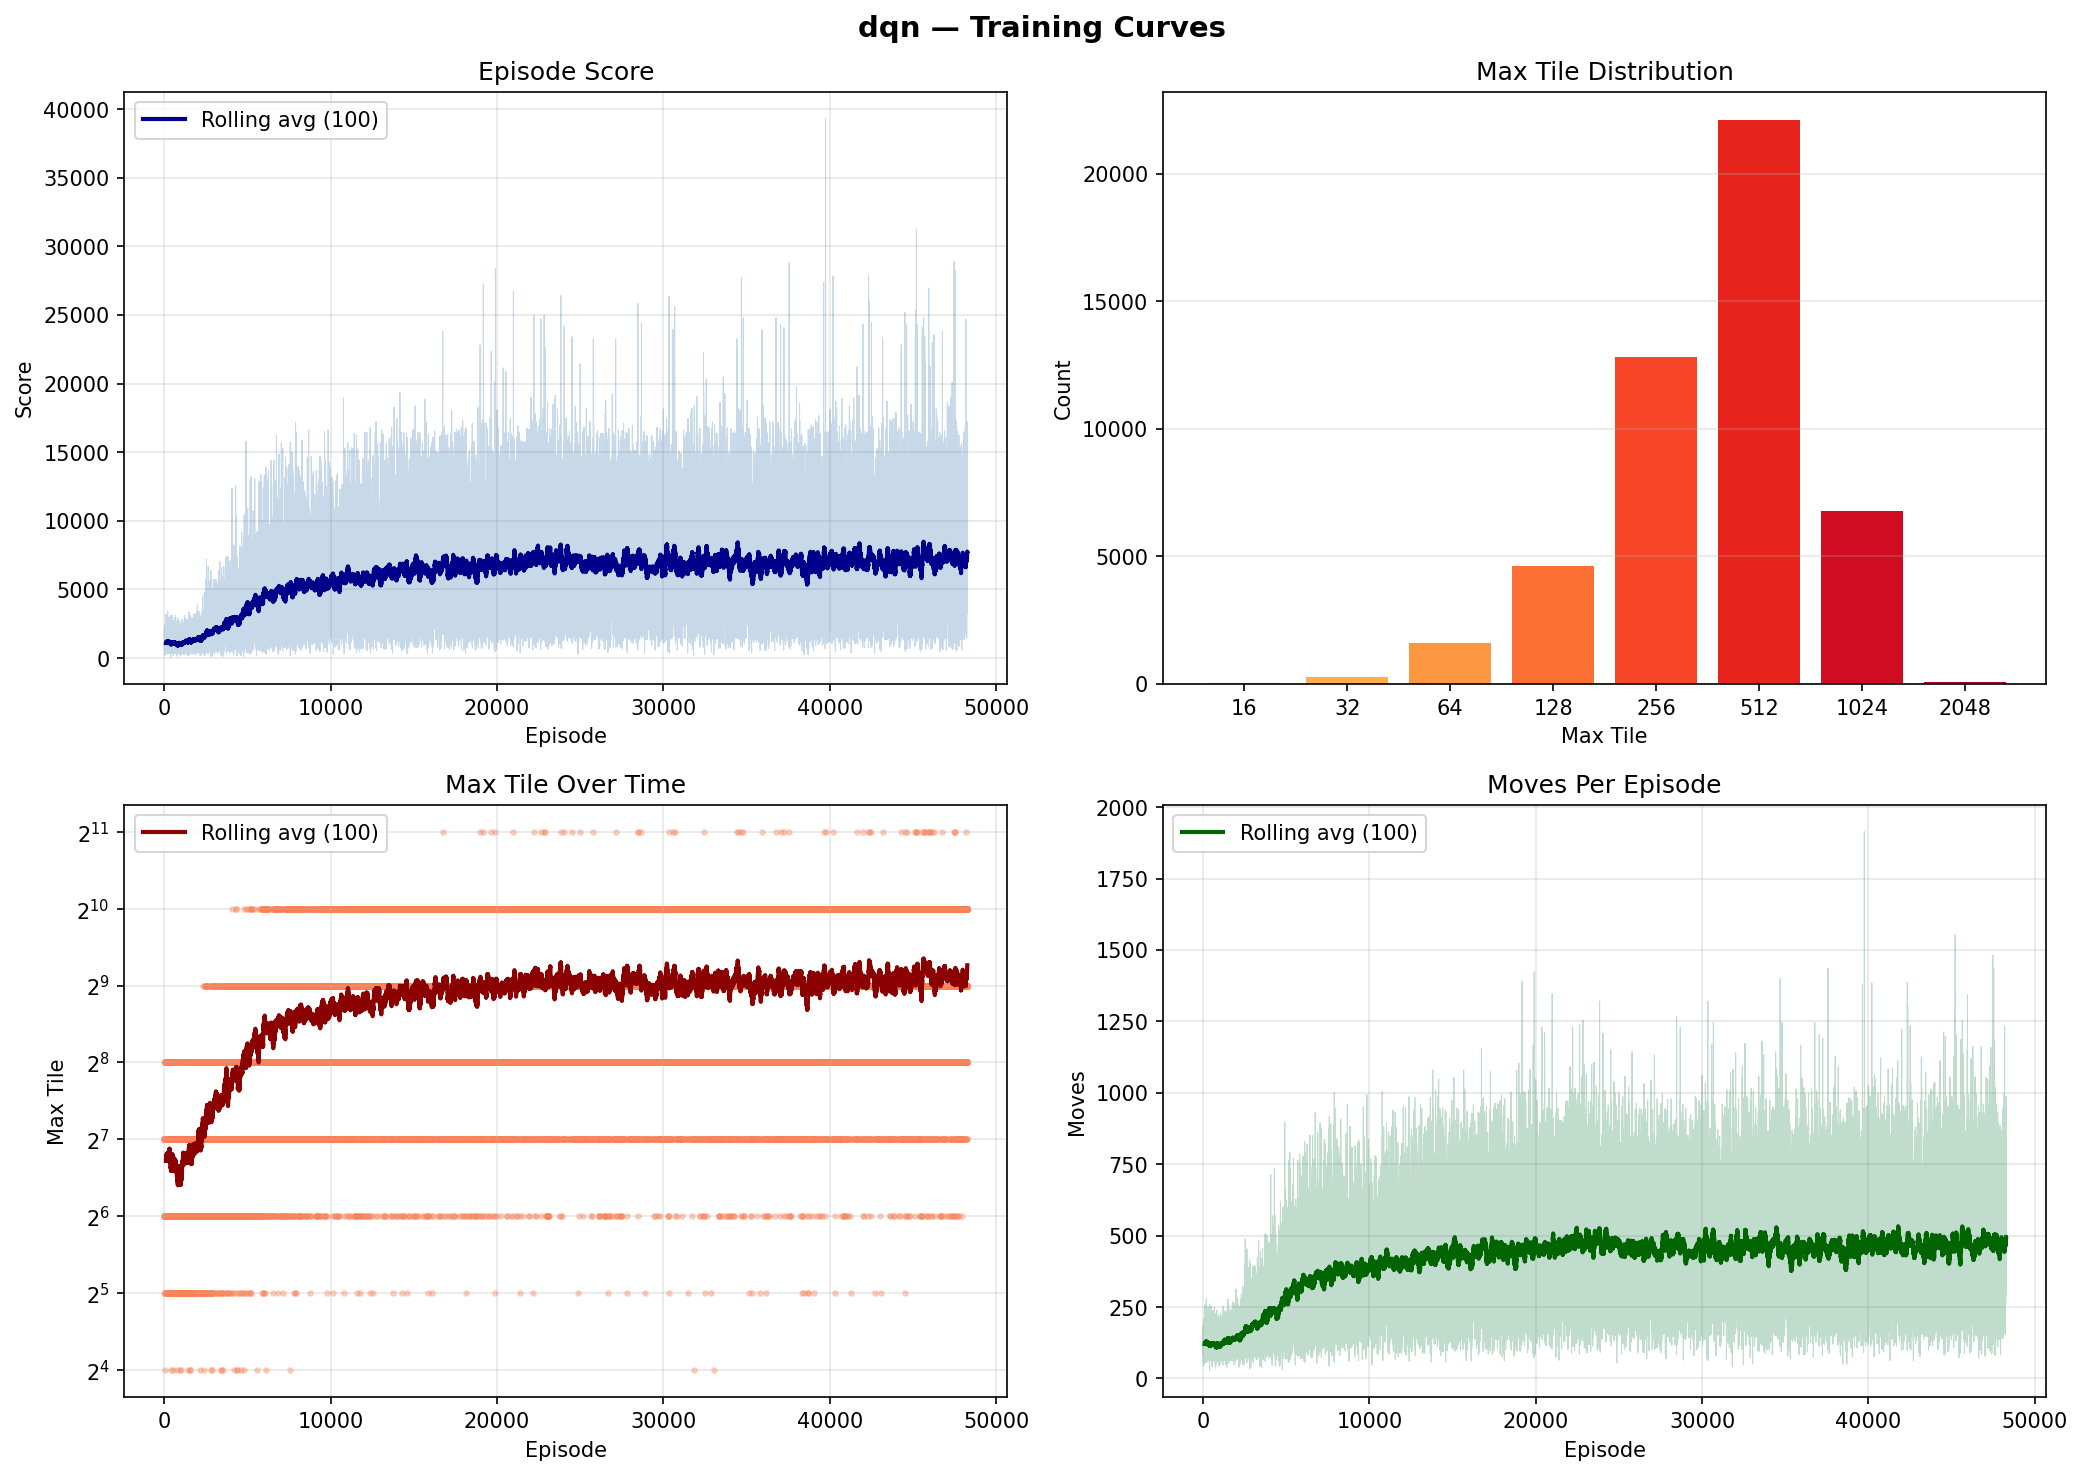
\includegraphics[width=\textwidth]{fig_dqn_5m.png}
        \caption{DQN (5M steps) --- avg 7,744}
        \label{fig:dqn}
    \end{subfigure}
    \hfill
    \begin{subfigure}[b]{0.48\columnwidth}
        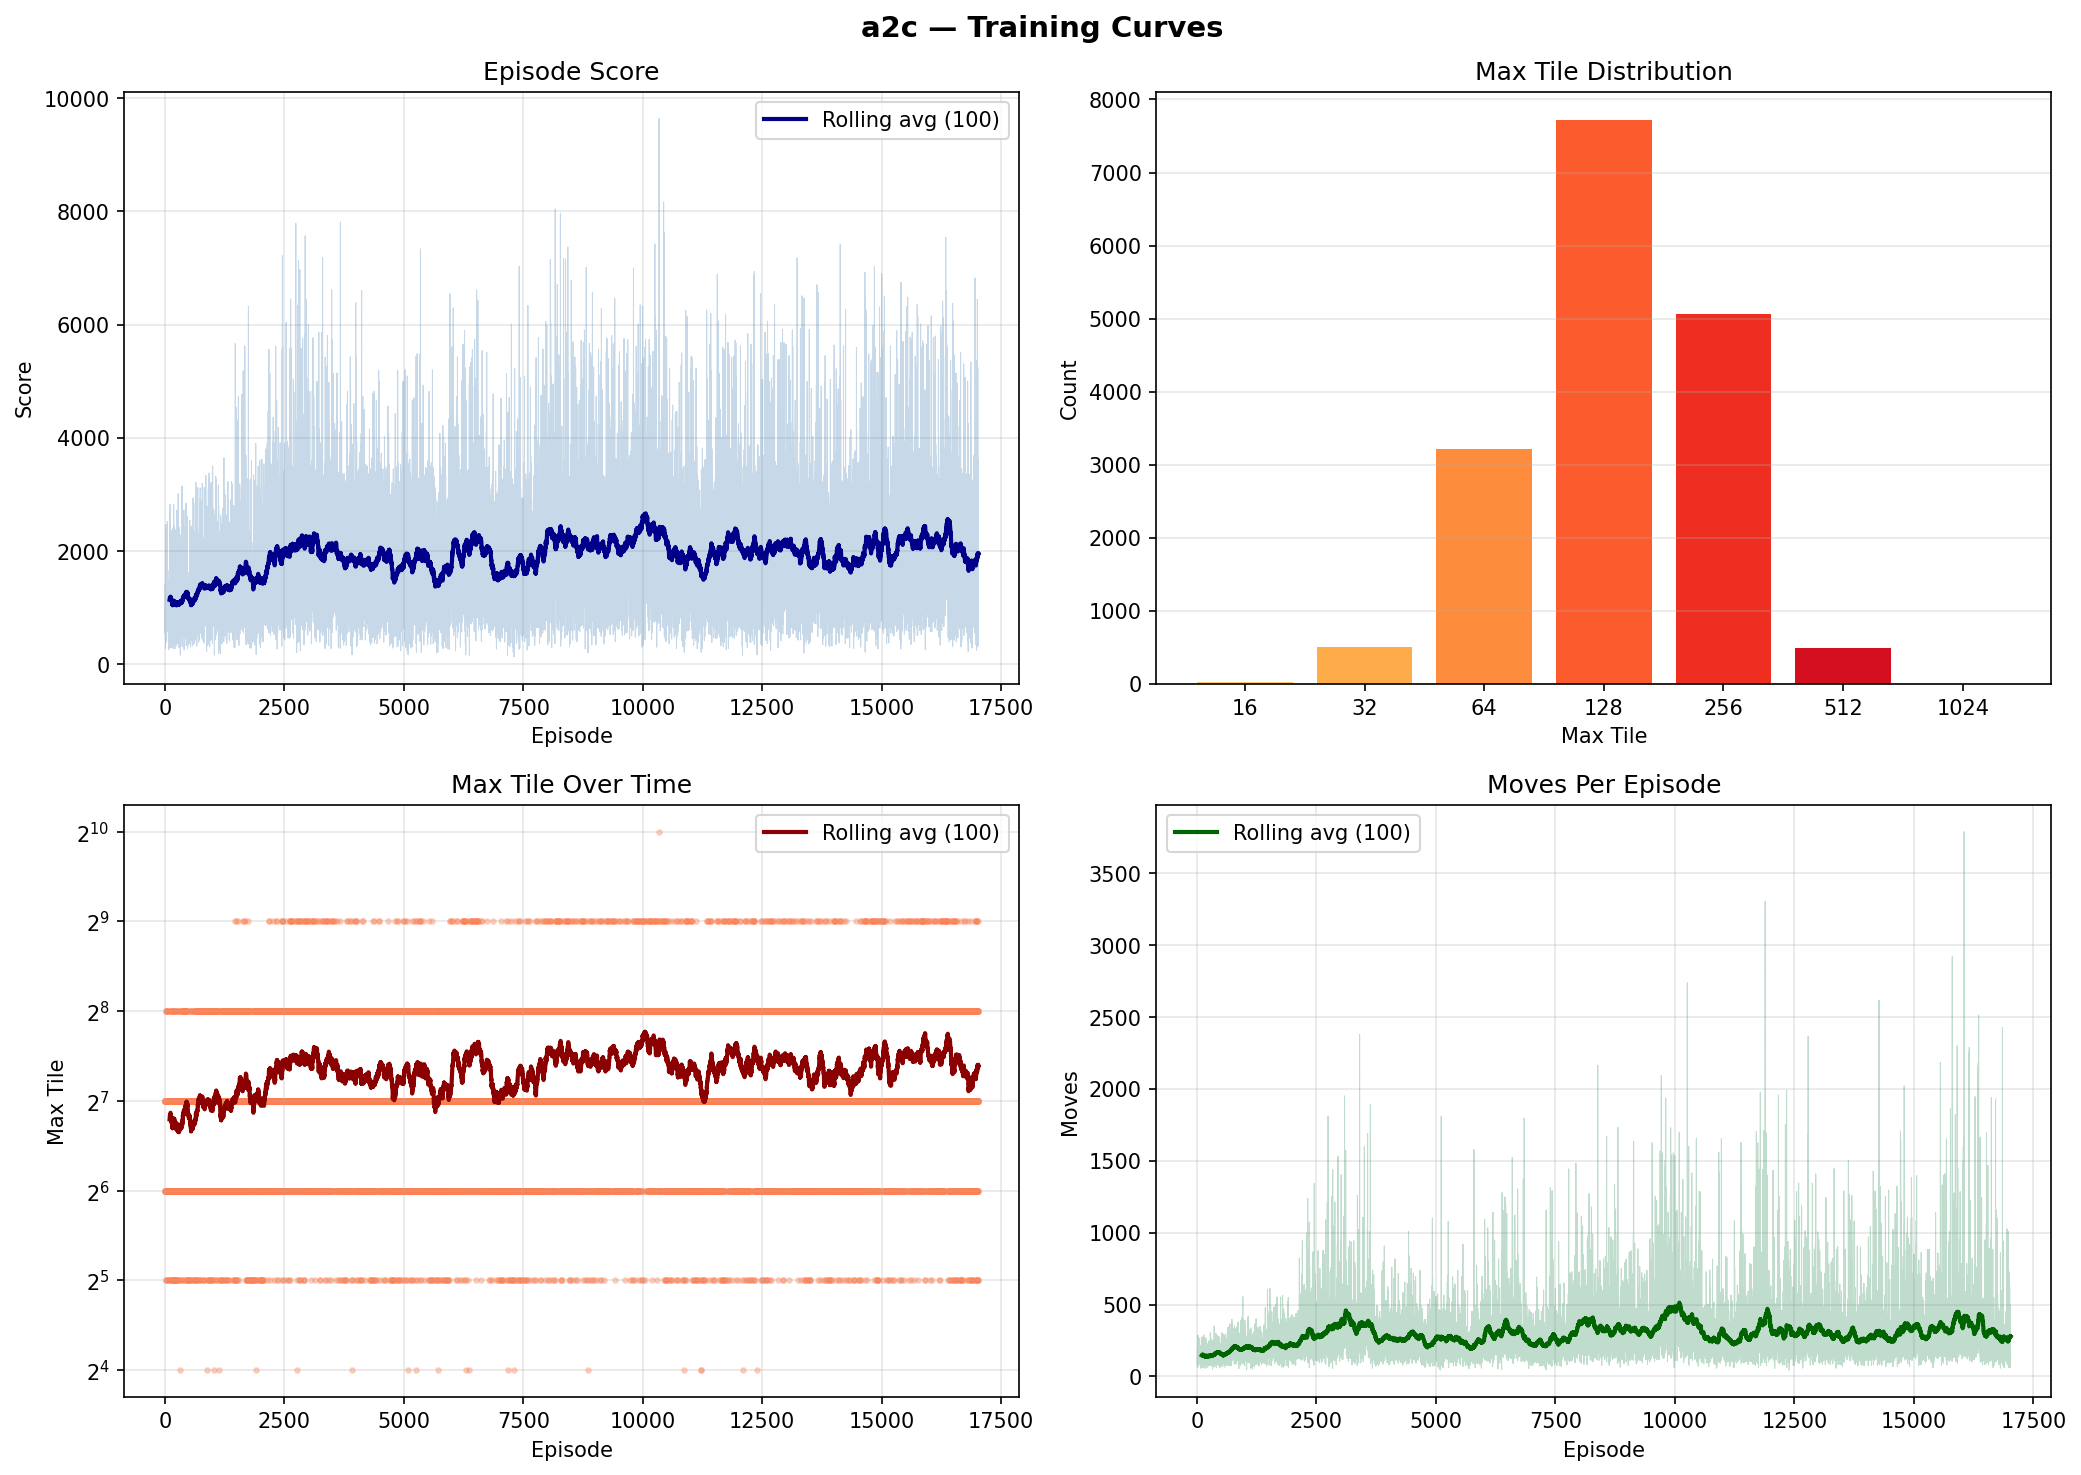
\includegraphics[width=\textwidth]{fig_a2c_5m.png}
        \caption{A2C (5M steps) --- avg 1,944}
        \label{fig:a2c}
    \end{subfigure}
    
    \vspace{4pt}
    
    \begin{subfigure}[b]{0.48\columnwidth}
        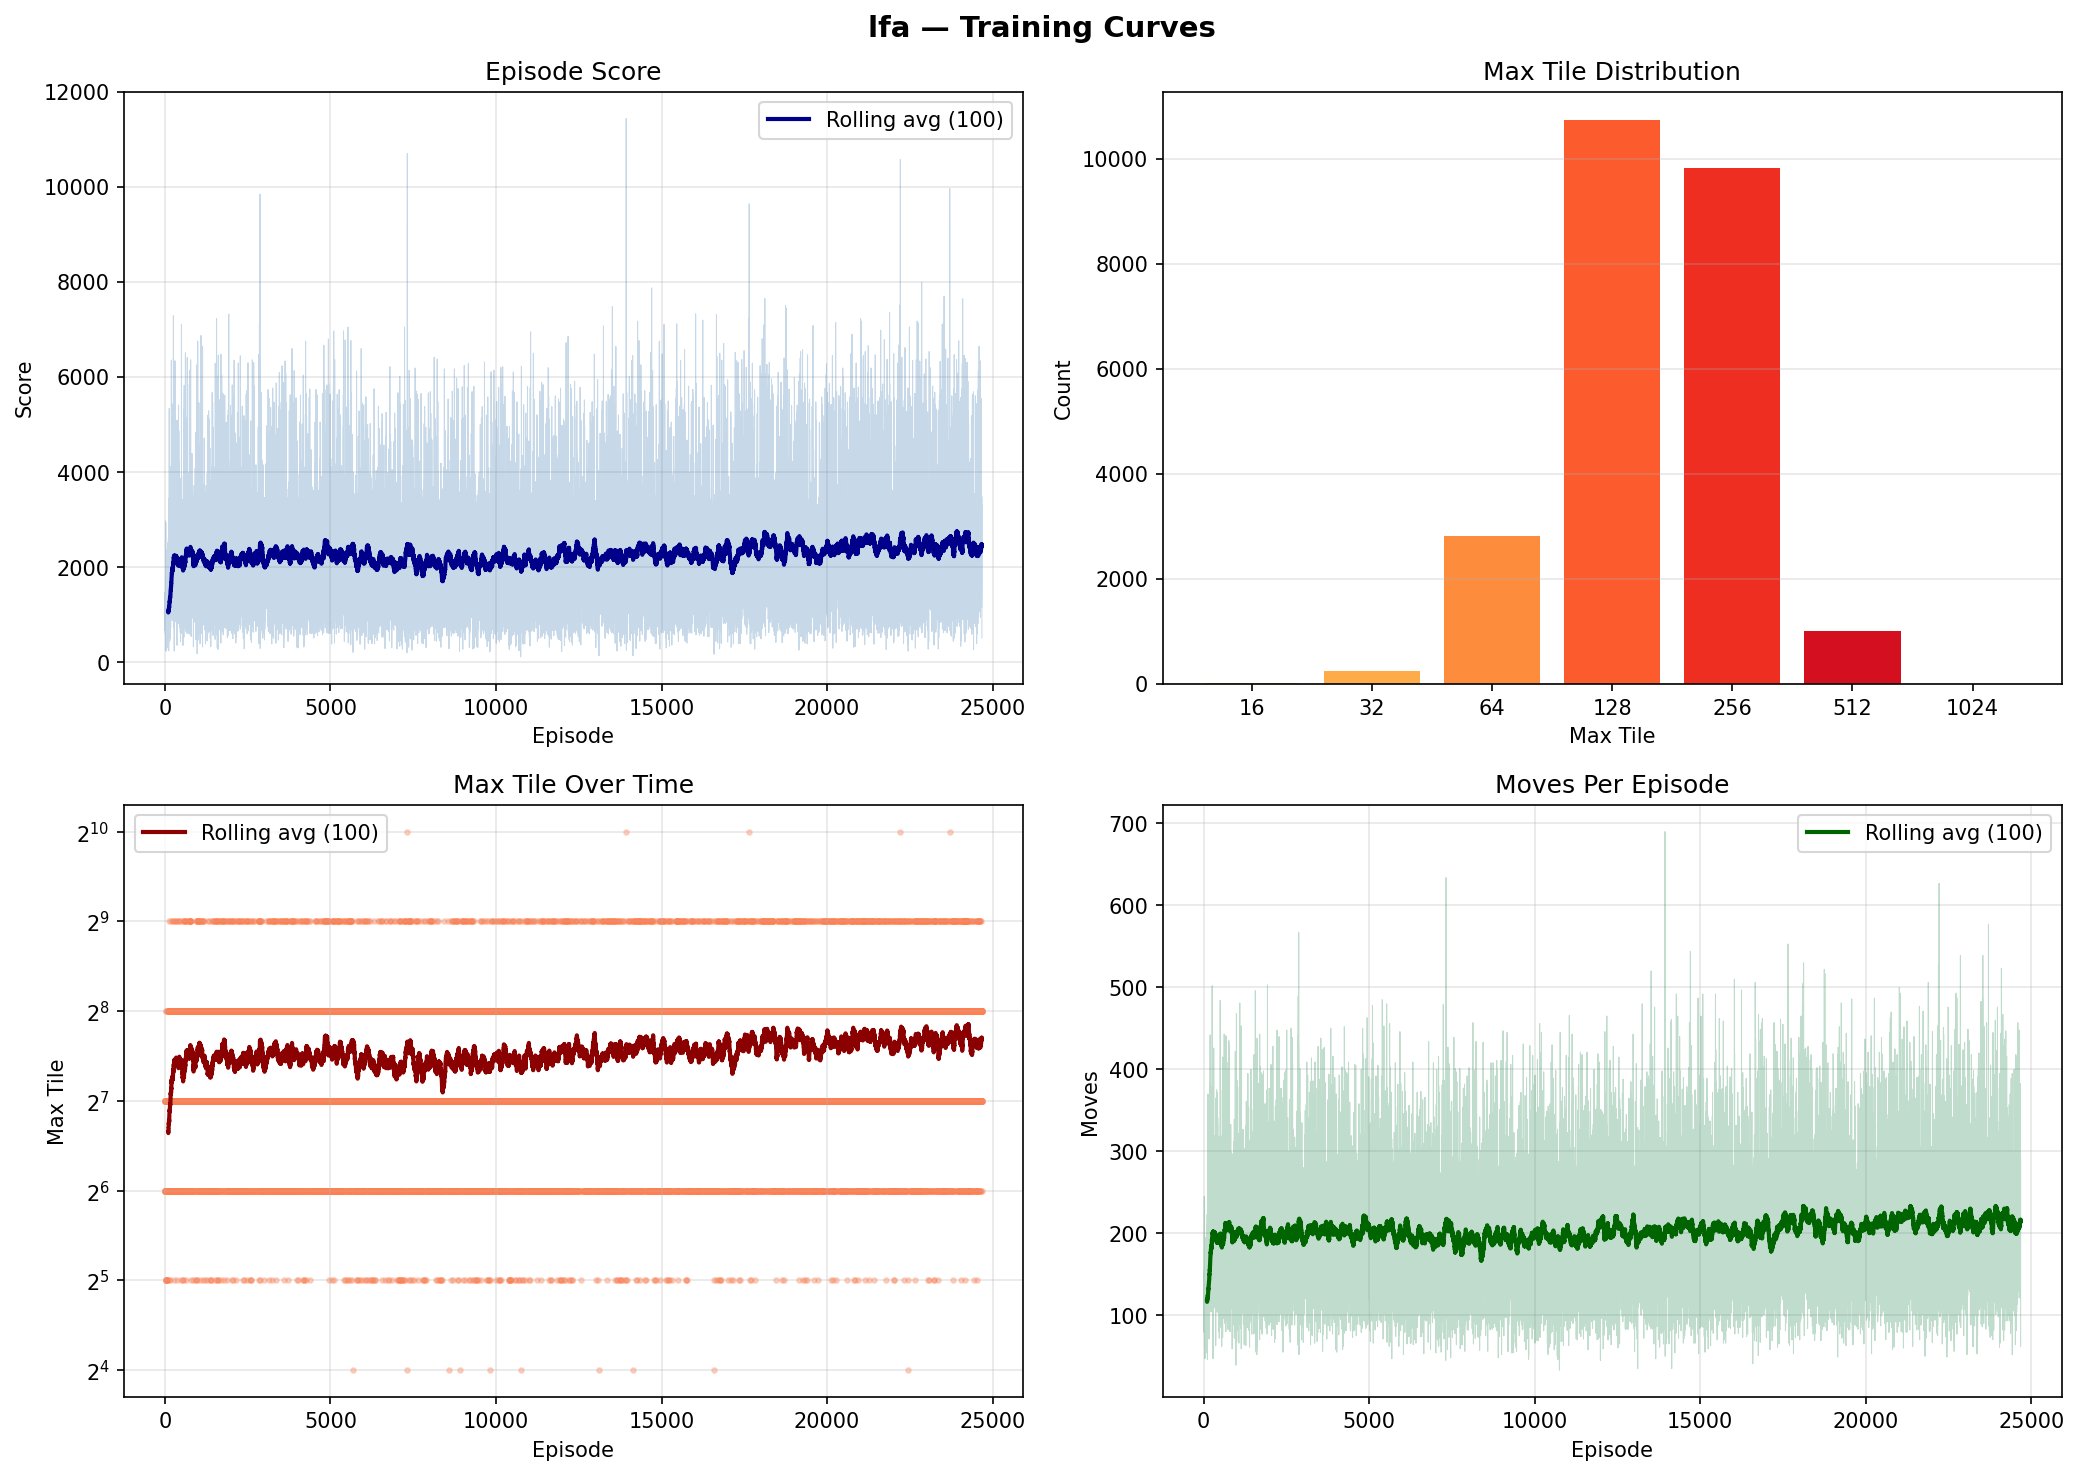
\includegraphics[width=\textwidth]{fig_lfa_5m.png}
        \caption{LFA (5M steps) --- avg 2,456}
        \label{fig:lfa}
    \end{subfigure}
    \hfill
    \begin{subfigure}[b]{0.48\columnwidth}
        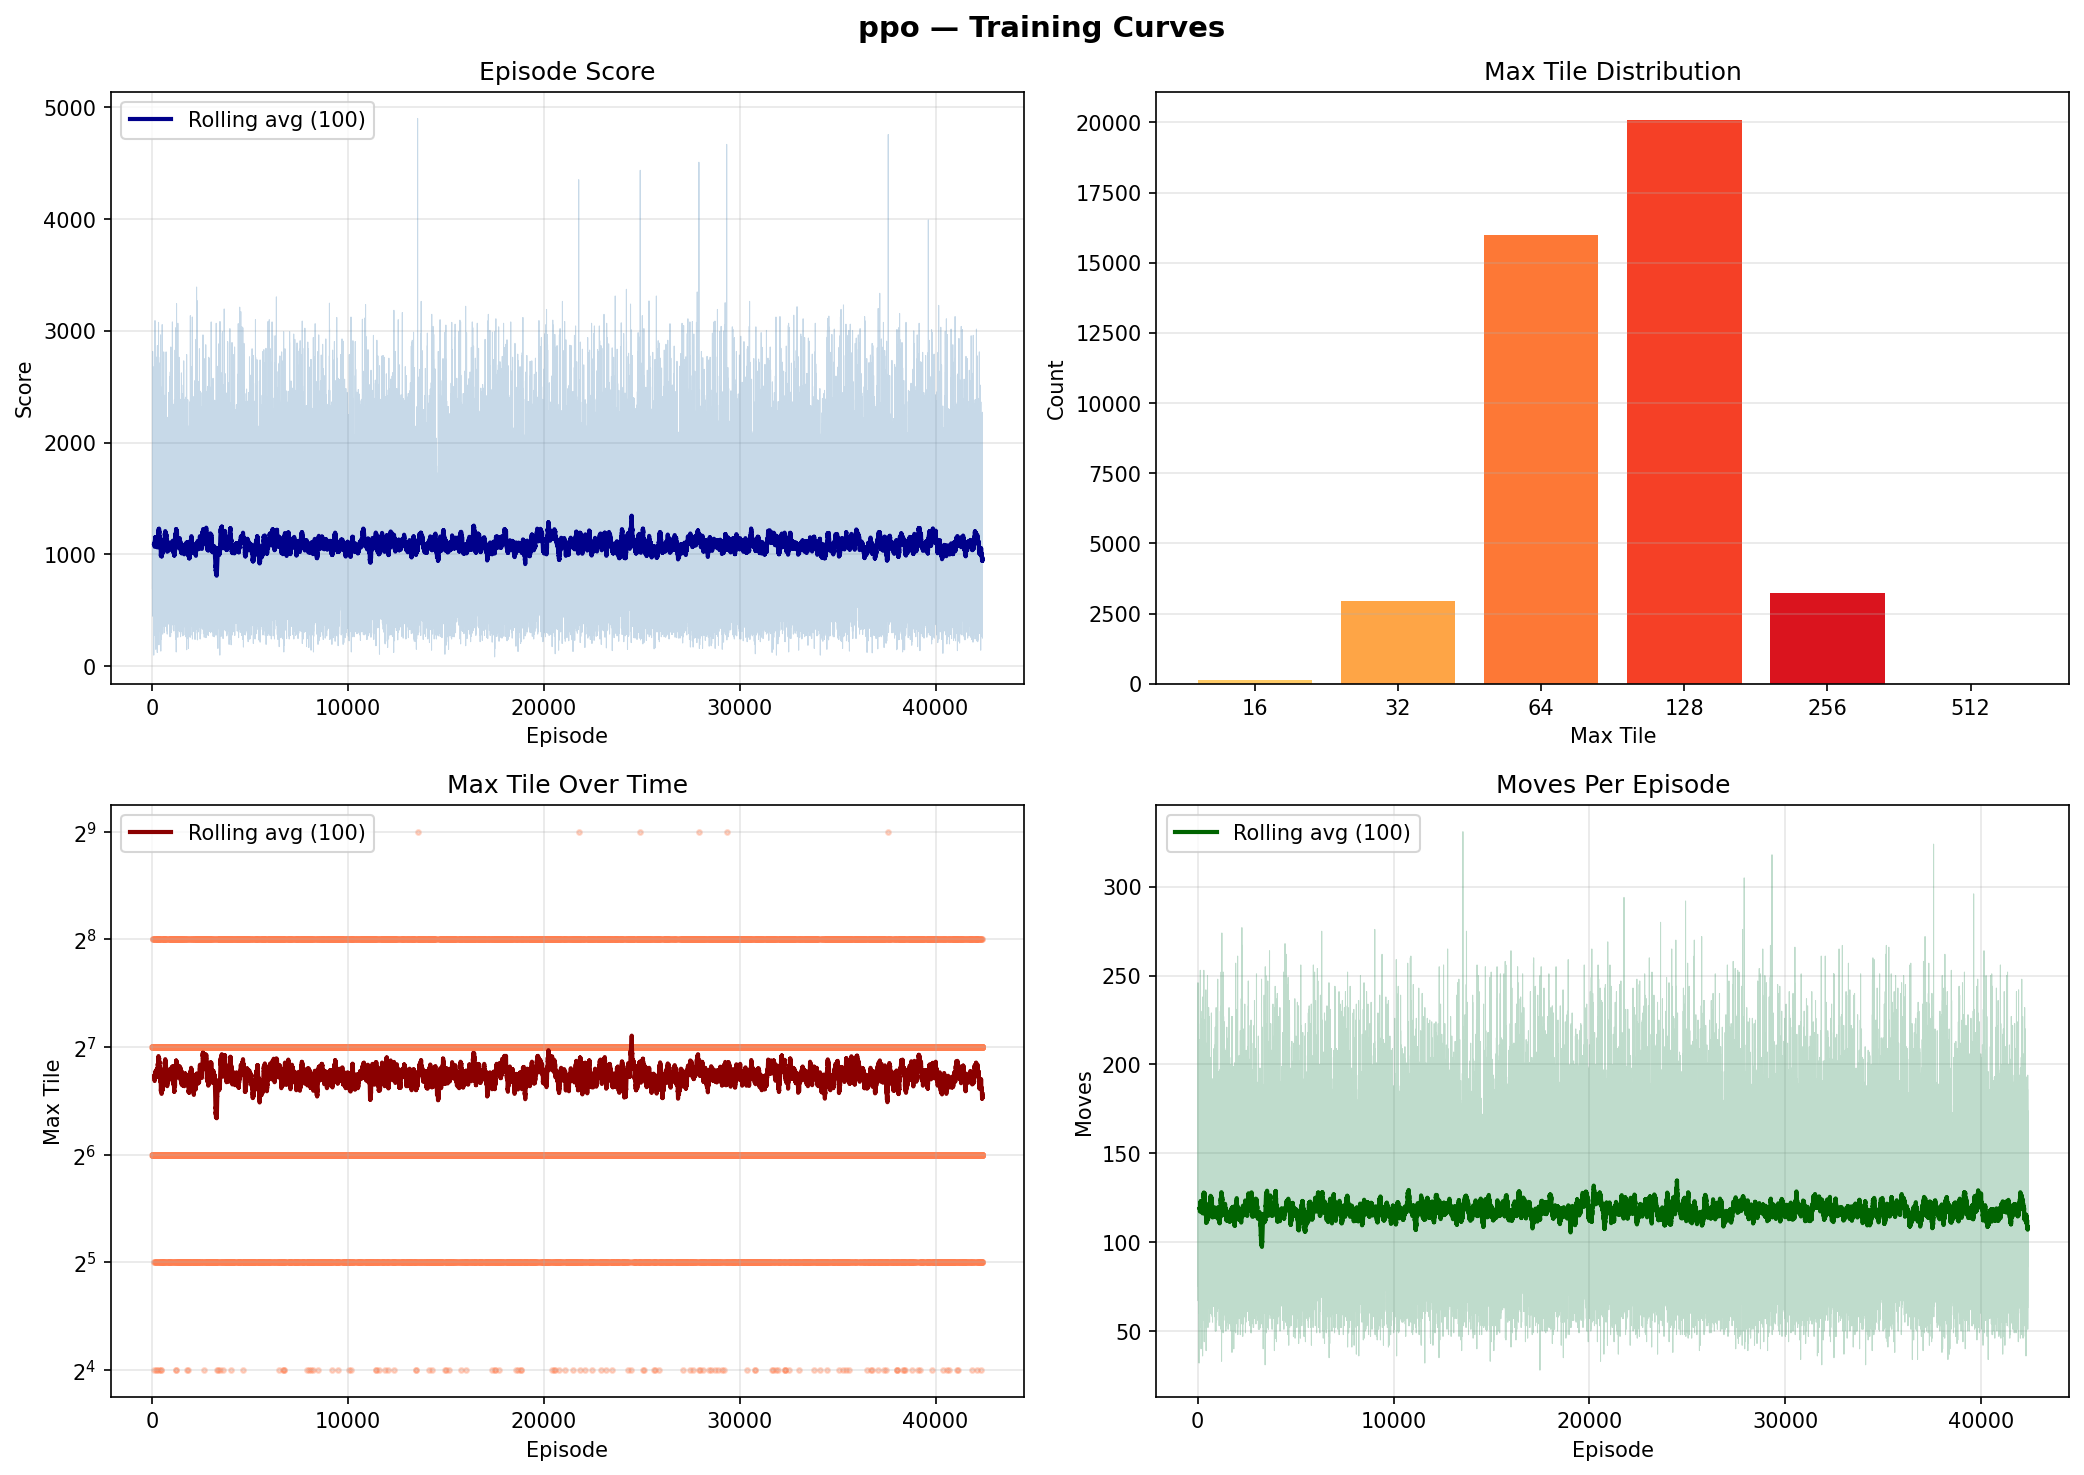
\includegraphics[width=\textwidth]{fig_ppo_5m.png}
        \caption{PPO (5M steps) --- avg 962}
        \label{fig:ppo}
    \end{subfigure}
    
    \caption{Training curves (5M steps, shaped reward).  DQN shows strong upward trajectory.  PPO flatlines near random baseline.}
    \label{fig:classical_curves}
\end{figure}

\begin{figure}[h]
    \centering
    \begin{subfigure}[b]{0.48\columnwidth}
        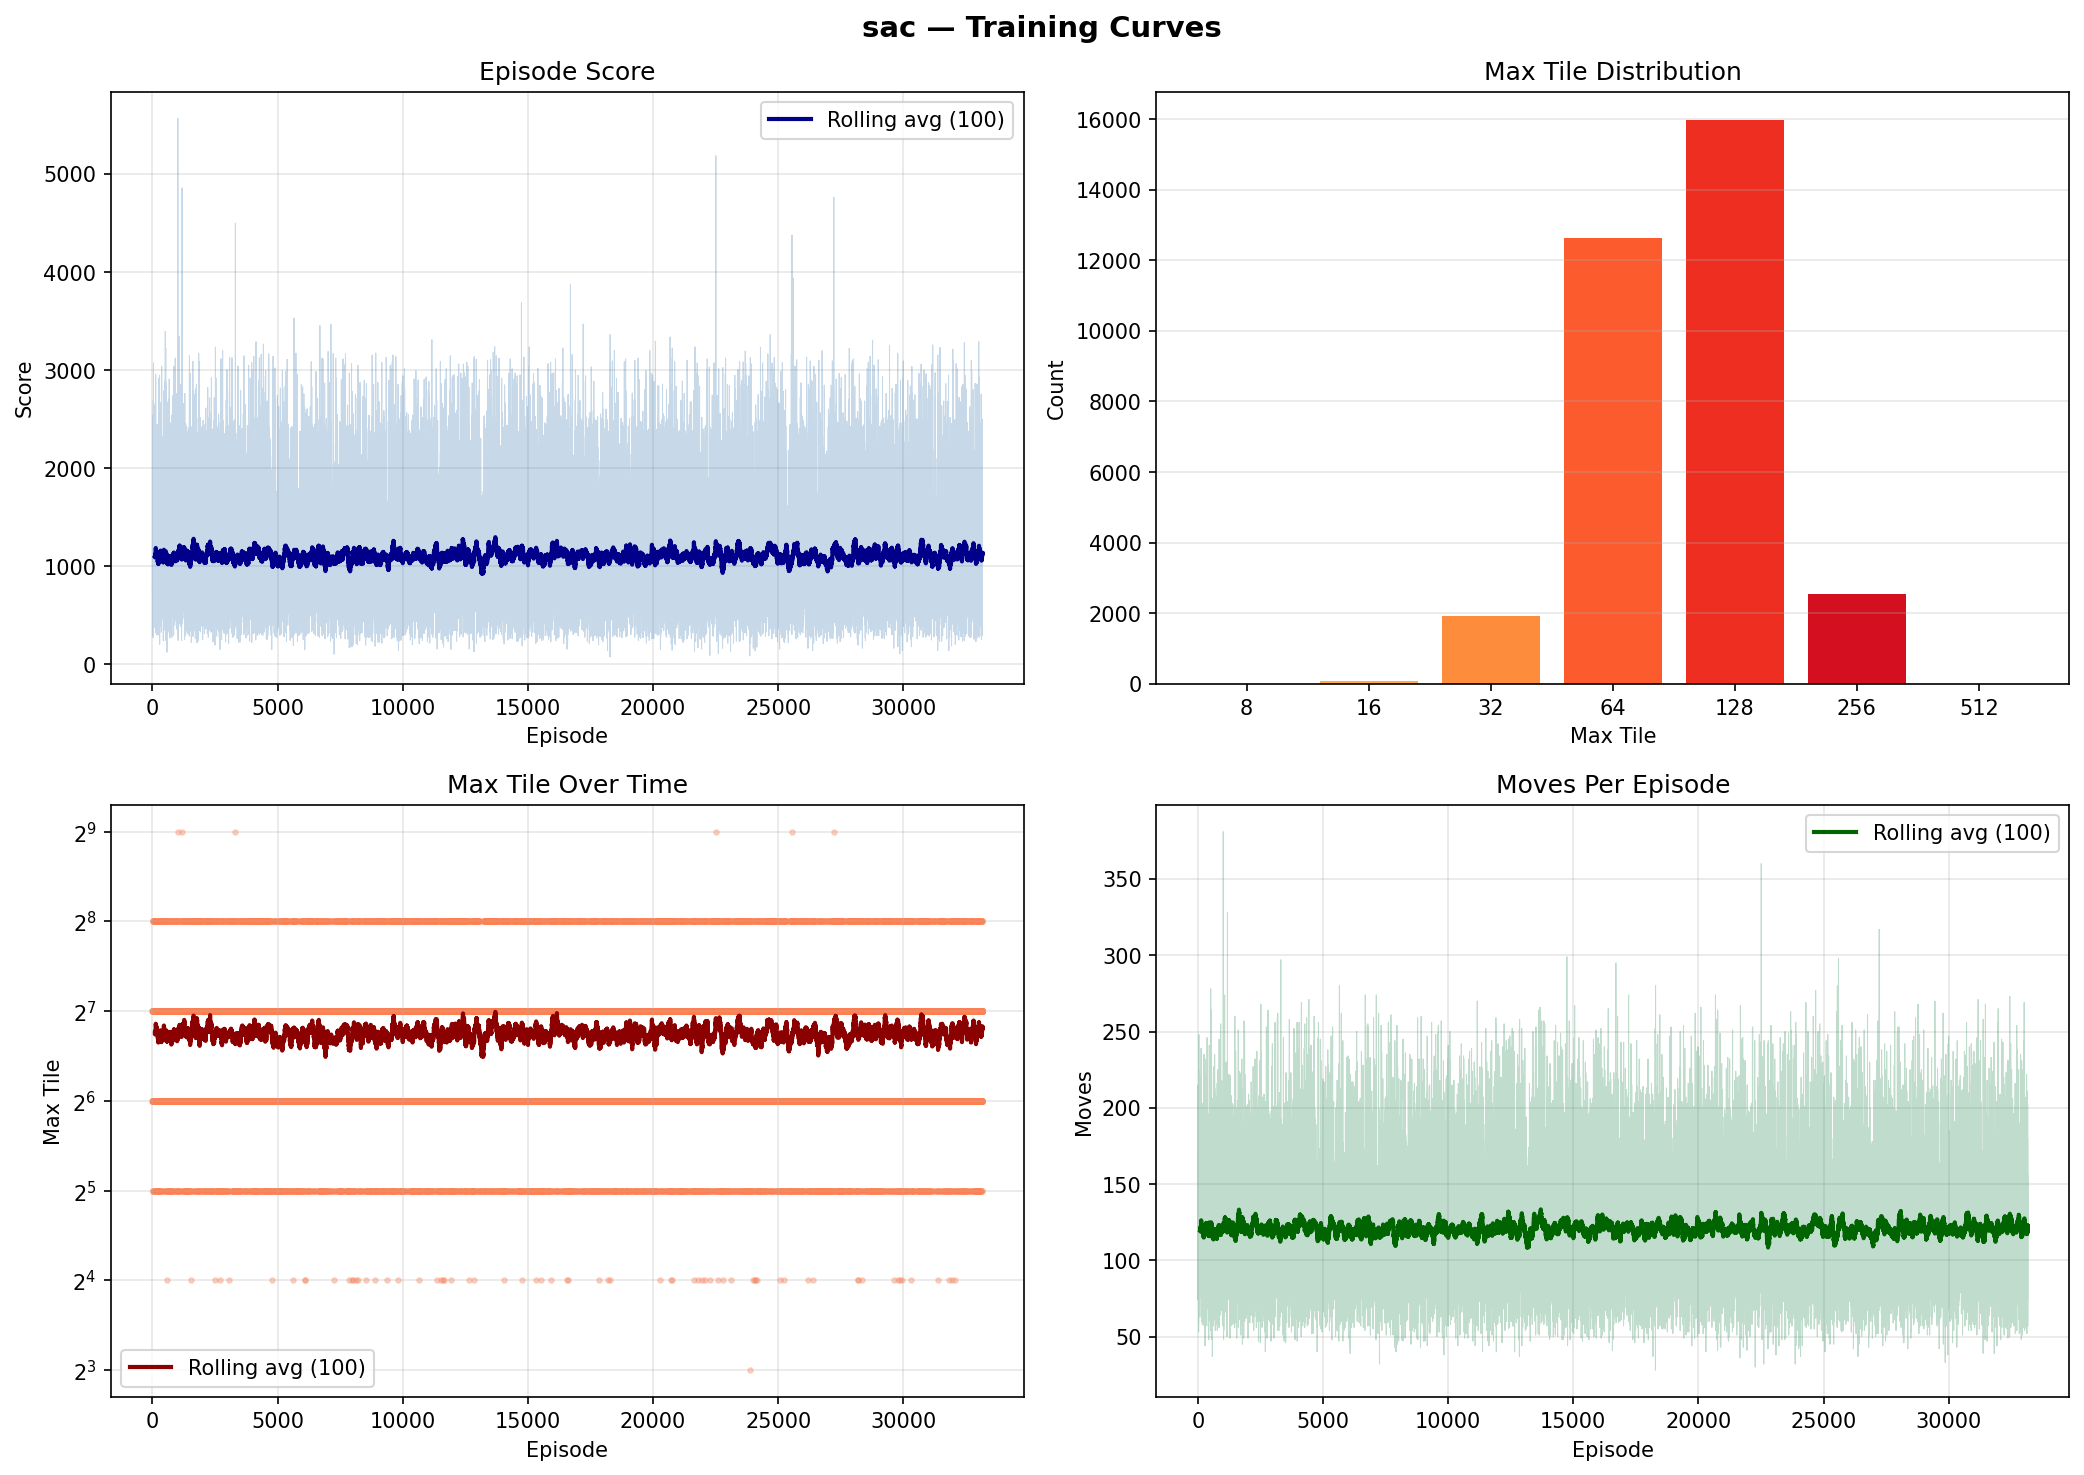
\includegraphics[width=\textwidth]{fig_sac_4m.png}
        \caption{SAC ($\sim$4M steps) --- avg 1,131}
        \label{fig:sac}
    \end{subfigure}
    \hfill
    \begin{subfigure}[b]{0.48\columnwidth}
        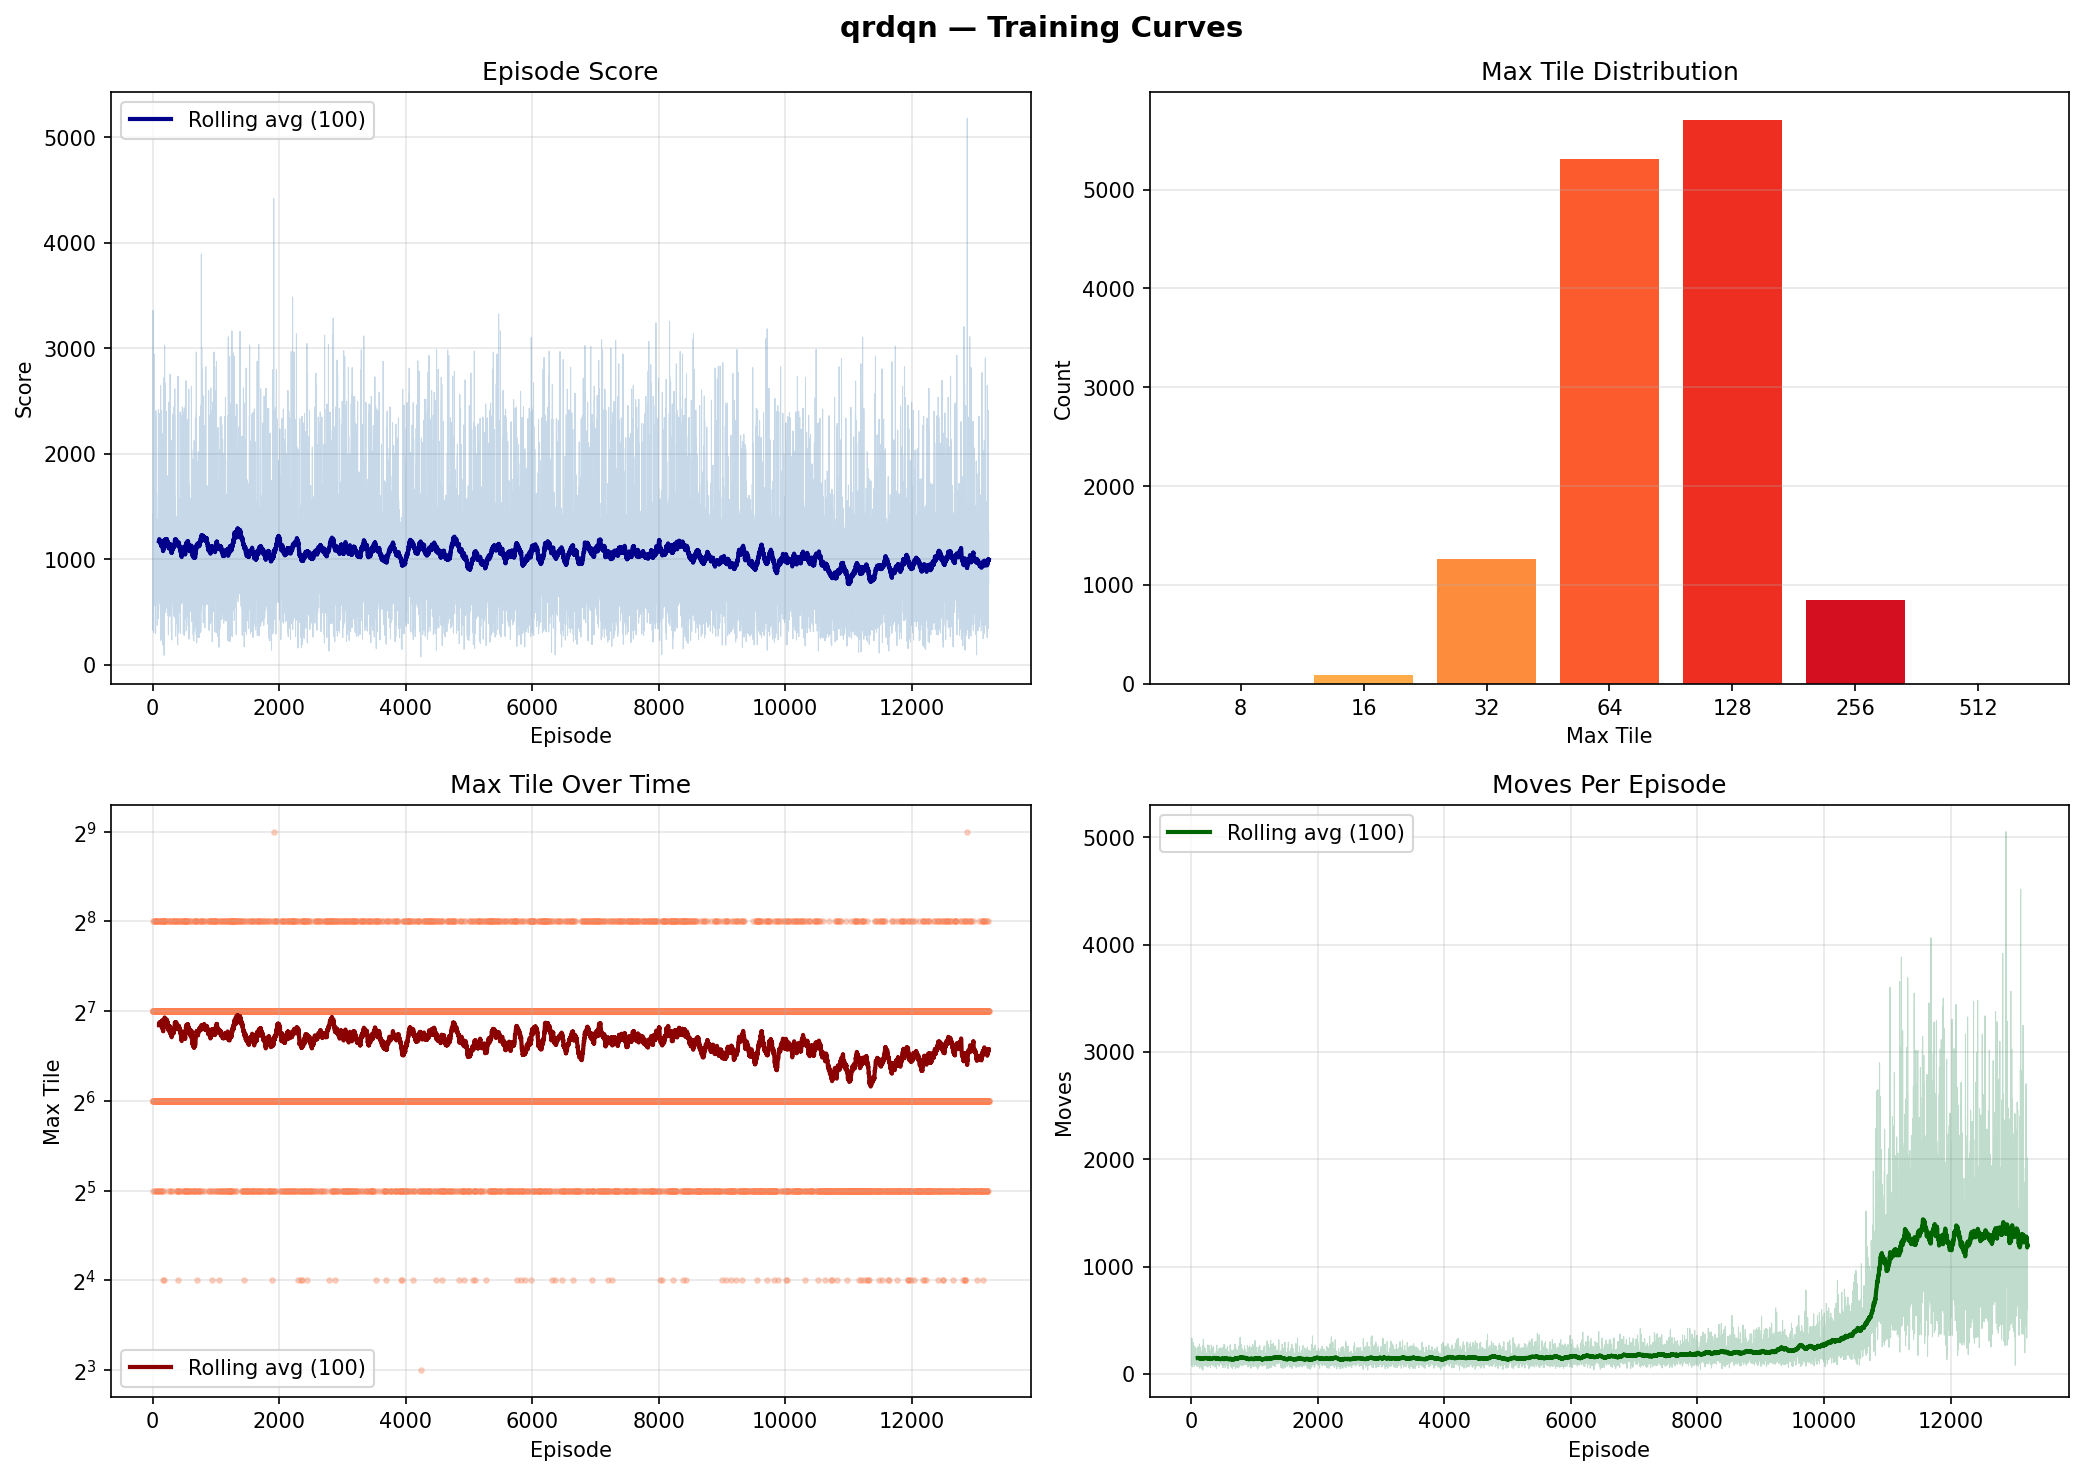
\includegraphics[width=\textwidth]{fig_qrdqn_5m.png}
        \caption{QR-DQN (5M steps) --- avg 995}
        \label{fig:qrdqn}
    \end{subfigure}
    \caption{SAC shows no learning trend despite off-policy replay.  QR-DQN's moves/episode explode (invalid-move loops).}
    \label{fig:more_curves}
\end{figure}

% ═══════════════════════════════════════════════════════════════════
% PAGE 4: Analysis, Discussion, Plan
% ═══════════════════════════════════════════════════════════════════

% ──────────────────────────────────────────────────────────────────
\section{Analysis \& Discussion}
\label{sec:analysis}
% ──────────────────────────────────────────────────────────────────

\subsection{Off-Policy Replay Is Decisive}

DQN's 100K-sample replay buffer lets it revisit rare high-scoring trajectories thousands of times, amplifying sparse reward signals.  At 5M steps DQN averages 7,744---a \textbf{3$\times$ lead} over the next-best agent.  On-policy methods (PPO, A2C) discard each trajectory after a single update, creating a chicken-and-egg problem: informative data requires a good policy, which requires informative data.

\subsection{Feature Engineering vs.\ Deep Learning}

LFA with \textbf{only 108 parameters} outperforms PPO (330K), QR-DQN (430K), SAC (330K), and the 494M-parameter LLM.  Its hand-crafted monotonicity and corner features provide a stronger inductive bias than CNNs learning from scratch.  However, LFA's linear capacity limits it below DQN---it cannot capture the complex tile interactions for the $1024\!\to\!2048$ merge.

\subsection{Scaling Reveals Divergent Trajectories}

Three distinct patterns emerge from $1\text{M}\!\to\!5\text{M}$ scaling (Table~\ref{tab:scaling}):
\begin{itemize}[nosep,leftmargin=*]
    \item \textbf{Strong scaling} (DQN, +174\%): Off-policy replay compounds with more diverse data.
    \item \textbf{Plateau} (LFA, +7\%): Linear model hits its representational ceiling.
    \item \textbf{Degradation} (PPO $-$12\%, QR-DQN $-$9\%): More training $\to$ worse policy.  PPO wastes probability mass on a fixed suboptimal policy; QR-DQN develops invalid-move loops (moves/episode explode from 200 to 1000+).
\end{itemize}

\subsection{GRPO: Format Before Strategy}

The LLM achieved 30--44\% format compliance (\texttt{<think>/<answer>}) after 300 steps with format-only rewards.  Key failure modes:
\begin{itemize}[nosep,leftmargin=*]
    \item \textbf{Reward hacking:} Length reward caused collapse---model generated filler text to maximize word count.
    \item \textbf{Gradient instability:} Grad norms exceeded 17,000 at step 297; KL spikes destabilized training.
    \item \textbf{Solution:} Staged rewards (format $\to$ direction $\to$ game), $\beta{=}0.04$ KL penalty, lr $10^{-6}$, gradient clipping 0.5.
\end{itemize}

\subsection{Inference Latency}

\begin{table}[h]
\centering
\caption{Inference Cost Per Move}
\label{tab:latency}
\setlength{\tabcolsep}{5pt}
\begin{tabular}{@{}lrrr@{}}
\toprule
\textbf{Agent} & \textbf{ms/move} & \textbf{Hardware} & \textbf{Params} \\
\midrule
LFA & $<$0.1 & CPU & 108 \\
PPO, A2C, SAC & $<$1 & GPU & 330K \\
DQN & 3.6 & GPU & 330K \\
QR-DQN & 4.2 & GPU & 430K \\
\textbf{LLM (GRPO)} & \textbf{1,500} & GPU & 494M \\
\bottomrule
\end{tabular}
\end{table}

The LLM is $\sim$400$\times$ slower but provides \emph{interpretable chain-of-thought reasoning}---each move is accompanied by a natural-language explanation.

% ──────────────────────────────────────────────────────────────────
\section{Conclusion \& Future Work}
\label{sec:conclusion}
% ──────────────────────────────────────────────────────────────────

\textbf{Key findings:}
\begin{enumerate}[nosep,leftmargin=*]
    \item \textbf{DQN dominates} (avg 7,744, tile 2048 in hunt mode) thanks to off-policy experience replay in this sparse-reward domain.
    \item \textbf{LFA (108 params) beats all deep on-policy methods}, demonstrating domain-specific features $>$ large neural networks.
    \item \textbf{On-policy methods fail to scale}: PPO and QR-DQN \emph{degrade} with 5$\times$ more training.
    \item \textbf{GRPO requires staged rewards}: simultaneous multi-reward training causes collapse.
    \item \textbf{Exploration is essential}: 5\% $\varepsilon$-noise breaks deterministic policy cycles at high-tile states.
\end{enumerate}

\textbf{Future work:}
\begin{itemize}[nosep,leftmargin=*]
    \item Complete SAC 5M training ($\sim$1M steps remaining)
    \item Staged GRPO: Stage~2 (+ game reward), Stage~3 (all rewards)
    \item Scaling curve evaluation at checkpoints 50K$\to$5M
    \item Multi-seed experiments (3 seeds $\times$ 7 agents) for error bars
    \item Hybrid LLM-MCTS for interpretability + search efficiency
\end{itemize}

% ──────────────────────────────────────────────────────────────────
\section*{Acknowledgment}
% ──────────────────────────────────────────────────────────────────

CS~5180 Reinforcement Learning, Prof.\ Robert Platt, Khoury College, Northeastern University.  All experiments: NVIDIA RTX 4060 (8\,GB VRAM), CUDA 12.6.

% ──────────────────────────────────────────────────────────────────
\begin{thebibliography}{00}
\bibitem{guo2025} D.~Guo \textit{et al.}, ``DeepSeek-R1,'' \textit{Nature}, vol.~645, 2025.
\bibitem{wen2025} Y.~Wen \textit{et al.}, ``RLVR Implicitly Incentivizes Reasoning,'' \textit{arXiv:2506.14245}, 2025.
\bibitem{saligram2025} P.~Saligram \textit{et al.}, ``2048: RL in Delayed Reward,'' \textit{arXiv:2507.05465}, 2025.
\bibitem{schulman2017} J.~Schulman \textit{et al.}, ``PPO Algorithms,'' \textit{arXiv:1707.06347}, 2017.
\bibitem{dabney2018} W.~Dabney \textit{et al.}, ``Distributional RL with QR,'' \textit{AAAI}, 2018.
\bibitem{haarnoja2018} T.~Haarnoja \textit{et al.}, ``Soft Actor-Critic,'' \textit{ICML}, 2018.
\bibitem{hu2025} L.~Hu \textit{et al.}, ``lmgame-Bench,'' \textit{arXiv:2505.15146}, 2025.
\end{thebibliography}

\end{document}
